%\documentclass[lettersize,journal]{IEEEtran}
\documentclass[journal]{IEEEtran}
\usepackage{amsmath,amsfonts}
\usepackage{algorithmic}
\usepackage{siunitx}
\sisetup{detect-all}
\usepackage{algorithm}
\usepackage{array}
\usepackage[caption=false,font=normalsize,labelfont=sf,textfont=sf]{subfig}
\usepackage{textcomp}
\usepackage{stfloats}
\usepackage{url}
\usepackage{verbatim}
\usepackage{graphicx}
\usepackage{cite}
\usepackage{hyperref} % for the url and hyperref
\usepackage{url}
\usepackage{booktabs} % For better table rules
\usepackage{tabularx} % For column width specification
\usepackage{pifont}% http://ctan.org/pkg/pifont
\newcommand{\cmark}{\ding{51}}%
\newcommand{\xmark}{\ding{55}}%
\hyphenation{op-tical net-works semi-conduc-tor IEEE-Xplore}
% updated with editorial comments 8/9/2021

\begin{document}

\title{TinyTapeout: A Shared Silicon Tapeout Platform Accessible To Everyone}

% contains serveral layouts of auhtors
% for anonymous authors
%\author{\IEEEauthorblockN{Anonymous Authors}


% layout 1
%\author{
%\IEEEauthorblockN{Alice Smith\IEEEauthorrefmark{1},
%Bob Jones\IEEEauthorrefmark{2}, and
%Charlie Brown\IEEEauthorrefmark{3}}
%\IEEEauthorblockA{\IEEEauthorrefmark{1}Department of Computer Science, University X\\
%Email: alice.smith@universityx.edu}
%\IEEEauthorblockA{\IEEEauthorrefmark{2}Department of Electrical Engineering, University Y\\
%Email: b.jones@universityy.com}
%\IEEEauthorblockA{\IEEEauthorrefmark{3}Department of Mathematics, University Z\\
%Email: charlie.brown@universityz.org}
%}

% layout 2
\author{
\IEEEauthorblockN{
    Matt Venn
}

\IEEEauthorblockA{TinyTapeout, YosysHQ\\
Email: matt@tinytapeout.com}
}


% The paper headers
\markboth{IEEE Solid-State Circuits Magazine}%
{Shell \MakeLowercase{\textit{et al.}}: TinyTapeout}

% to be complemented once there is DOI and so on
%\IEEEpubid{0000--0000/00\$00.00~\copyright~2024 IEEE}
% Remember, if you use this you must call \IEEEpubidadjcol in the second
% column for its text to clear the IEEEpubid mark.

\maketitle

%\begin{abstract}
%The abstract goes here
%\end{abstract}

% to be completed or removed
\begin{IEEEkeywords}
ASIC, Multi Project Chip, Open Source Silicon, TinyTapeout.
\end{IEEEkeywords}

\section{Introduction}
\label{sec:introduction}
\IEEEPARstart{T}{inyTapeout} is a multi project chip platform that makes it easier and cheaper to get Application Specific Integrated Circuit (ASIC) designs manufactured.

Open source tools and Process Design Kits (PDK~\cite{pdk}) are used so no licenses or Non Disclosure Agreement (NDAs) are required. As the tools run on remote cloud servers no software needs to be installed locally on the user's machine. As long as the template structure is followed, however, TinyTapeout does support the use of proprietary tools.

Each TinyTapeout ASIC production run sees around 400 open source designs multiplexed to 24 General Purpose Input/Output (GPIO) pins. After manufacture the resulting chip is mounted to a demonstration board for ease of testing. Each chip contains a copy of every design, which can be selected and tested in turn.

At the same time each participant submits documentation for their design, which used to create a printable datasheet~\cite{datasheet} along with an online project index at TinyTapeout.com/runs/~\cite{tinytapeoutruns}. The datasheet helps participants explore other designs on the chip in addition to their own.

By separating the cost of area on a silicon wafer and the finished physical chip, the TinyTapout participant group is able to share the cost of chip packaging and circuit board manufacture while still being able to test and measure all the designs on the chip. For use in educational settings it is possible for multiple students to submit individual designs while sharing the finished chips and circuit boards, reducing the cost still further.

Each TinyTapeout tile (Fig.~\ref{fig:render_cells_in_use}) is approximately $160 \times \qty{100}{\micro\meter\squared}$. This provides enough room for around 1,000 logic gates when built upon the SkyWater 130nm open source PDK. Multiple tiles can be interconnected to enable larger designs, while analog and mixed signal support is on the roadmap for the next shuttle.

Community engagement in TinyTapeout has been strong, with 756 designs submitted over the first five shuttles. A curated selection of projects is provided in section~\ref{sec:silicon_showcase}.
An online chat server for participants has 1,000 members with 1,600 subscribers to the project's mailing list. Individuals submitting designs to TinyTapeout tend to self identify as hobbyists, students, and teachers, as shown in Fig.~\ref{fig:TT04_submitters}.

The first~\cite{firstshuttle} TinyTapeout production run, which was provided as a free and experimental effort with a total of 152 designs, was submitted to the seventh Google-sponsored~\cite{googlesponsored} lottery based Multi Project Wafer (MPW) shuttle in September 2022.
The next four shuttles combined a total of 582 designs, all sponsored by and manufactured through the Efabless~\cite{efabless} chipIgnite MPW service. Table~\ref{tab:tinytapeout} shows a summary of all TinyTapeout shuttle runs to date.

The rest of this paper will detail the TinyTapeout design flow, multiplexer evolution, circuit board design, the results of post production silicon testing, and the project's next steps.

\begin{table*}[!t]
\centering
\caption{Statistics from all TinyTapeout shuttle runs to date.}
\label{tab:tinytapeout}
\begin{tabularx}{\textwidth}{@{}l *{6}{X}@{}}
\toprule
\textbf{Run} & \textbf{Launched} & \textbf{Shuttle} & \textbf{Designs} & \textbf{Estimated delivery date} & \textbf{Architecture} \\
\midrule
TT01 & 2022-08-17  & MPW7  & 152 & n/a        & Scan chain \\
TT02 & 2022-11-09  & 2211Q & 165 & 2024-01-30 & Scan chain \\
TT03 & 2023-03-01  & 2304C & 249 & 2024-02-28 & Scan chain inverted clock \\
TT04 & 2023-07-01  & 2309  & 143 & 2024-04-15 & Mux \\
TT05 & 2023-09-11  & 2311  & 174 & 2024-05-12 & Split Mux \\
TT06 & 2024-02-01  & 2404  & TBD & 2024-11-30 & Split Mux \\
\bottomrule
\end{tabularx}
\end{table*}

\begin{figure}[!t]
\centering
\includegraphics[width=\columnwidth]{./Figs/gh action gds layout.png}
\caption{A 2-D render of a single TinyTapeout tile.}
\label{fig:render_cells_in_use}
\end{figure}

\begin{figure}[!t]
\centering
\includegraphics[width=\columnwidth]{./Figs/about our community pie chart.png}
\caption{Tiny Tapeout 04 participant self identification.}
\label{fig:TT04_submitters}
\end{figure}

\section{Design Flow}
\label{sec:design_flow}

Tiny Tapeout designs are primarily developed in the Verilog Hardware Description Language (HDL) or Wokwi~\cite{wokwi}.
Wokwi is a web based visual schematic editor for hardware description, designed as an easier way for individuals with no prior HDL experience to get started.
The TinyTapeout website~\cite{tinytapeout} includes a basic Wokwi getting started guide, demonstrating how to use the tool to draw circuits, which is made available in English and Spanish.

The design flow has the participant create a GitHub~\cite{github} source code repository based on provided templates then add their ASIC design. This triggers automated tests and the generation of binary layout files in GDSII~\cite{gds}. If all tests pass and the binary layout files are correctly generated, the design is then submitted to a quarterly shuttle for production in silicon.

The TinyTapeout GitHub templates\cite{verilogtemplate} make use of GitHub Actions\cite{githubactions}---an automatic continuous integration system triggered every time the repository is updated. This reduces duplicated effort and makes it possible for TinyTapeout to support large numbers of participants without excessive technical overhead.

There are four main jobs in the continuous integration system:

\begin{enumerate}
	\item GDS: installs OpenLane\cite{openlane} and the SkyWater Sky130\cite{skywaterpdk} PDK, builds the binary layout files, and generates a summary of the design (Fig.~\ref{fig:summary_table_GDS_job}). The summary includes utilization, standard cells used, a 2-D render (Fig.~\ref{fig:render_cells_in_use}) and an interactive 3-D viewer (Fig.~\ref{fig:interactive_3D_viewer}).
This job can also optionally run a gate-level verification of the design.
	\item Verification: installs the YosysHQ open source Computer-Aided Design (CAD) suite, which includes many common electronic design automation (EDA) tools; uses iVerilog\cite{iverilog} and cocotb\cite{cocotb} to run included testbenches.
	\item Documentation: generates a preview of the documentation.
	\item Precheck: runs Design Rule Check (DRC) tests to ensure the design can be integrated into the multi project chip.
\end{enumerate}

Successful GDS, Documentation, and Precheck job completion are all required for a design to be submitted to a shuttle for production.
Verification is optional but highly encouraged. Submissions designed in Wokwi are able to make use of its integrated truth table testing system\cite{automatedtesting}.

While the TinyTapeout continuous integration system can be run entirely in the user's web browser, it is also possible to install a local copy of the tools\cite{localinstall} on a participant's computer. Locally installed tools can help to reduce the time between design iterations, especially for the test and verification jobs.

\begin{figure}[!t]
\centering
\includegraphics[width=\columnwidth]{./Figs/gh action cell stats.png}
\caption{A summary table from the GDS continuous integration job.}
\label{fig:summary_table_GDS_job}
\end{figure}

\begin{figure}[!t]
\centering
\includegraphics[width=\columnwidth]{./Figs/gh action gds 3d view.png}
\caption{The interactive 3-D viewer.}
\label{fig:interactive_3D_viewer}
\end{figure}

\section{Scanchain architecture}
\label{sec:scanchain_arch}
%TinyTapeout started as an experiment in fitting as many designs as possible into the 10 mm2 available on the Google lottery shuttles. As a fast proof of concept, a scan chain was chosen. Each design had 8 inputs and 8 outputs. Clock and reset were optional and not treated specially. The chain was formed of scan flops[13], a type of flip flop with an integrated multiplexer at its input.
%
%
%Figure shows 500 designs connected in a chain for TT01, with the scan chain driver in the lower left corner. A dense power distribution network was needed for so many small designs.
%
%
%Figure shows a simplified view of 2 designs in the chain.
%
%
%Each design sends data into the scan flops secondary input and receives input from the output of the flop via a latch. The chain is built[14] by sending data from the output of the previous scan flop into the next scan flops’s primary input.
%
%
%This arrangement allows the loading of data into any of the designs, and then capturing the output and clocking that through the rest of the chain to the output.
%
%
%While relatively easy to implement, the downside is the latency. The more designs in the chain, the longer it takes to send and receive data.
%
%
%Assuming a 50MHz scan chain clock, 250 designs with 8 inputs and 8 outputs, the maximum refresh rate is 50M / (8 * 250) = 25kHz.
%
%
%Another concern is hold violations due to the large number of serially connected flops and potentially large clock skews due to long signal wires. This was mitigated by:
%
%
%* Reclocking the output data with a negedge flop, providing more hold margin
%* Driving the latch and scan signals separately, and with a configurable delay,
%* Keeping wires between designs short by snaking them through the grid.
%
%
%To further reduce the risk of failure, 3 independent methods of driving the chain are provided:
%
%
%1. External - all the signals are available as GPIO pins on the chip. This safest option is the default.
%2. Internal - an internal scan chain driver runs the chain and copies the data to and from 16 GPIOs.
%3. Logic analyser. The Caravel[15] harness provided by Efabless contains a RISCV co-processor with a firmware driven logic analyser. The logic analyser was connected as a 3rd possible way to drive the chain and hence access all designs from firmware.
%
%
%After static timing analysis (STA) it was discovered that the clock duty cycle would increase slightly at each of the 500 sequential clock drivers. This is because P MOSFETs are weaker than N MOSFETs, so for a balanced drive the P MOSFET needs to be substantially larger than the N. To save space, the P mosfet is typically undersized in standard cells, and so the rising clock edge is always slightly slower. This effect limits the maximum clock speed as eventually the clock duty cycle tends to 100%, but faster speeds are possible by starting with a lower duty cycle. With a 50% duty cycle a 30MHz maximum clock is expected, limiting the refresh rate to 7kHz.
%
%
%Alternative:
%
%
%After static timing analysis (STA) it was discovered that the clock duty cycle could change substantially due to the 500 sequential clock drivers. Depending on the exact capacitance between each design, the clock duty cycle could either increase or decrease, with this effect magnified over the chain.
%
%
%TT01’s scan chain was embedded into each design, which created the risk that a user could unintentionally break it, and break the rest of the chain. This risk was mitigated by formally[16] proving the chain was present in the submitted design. For TT02 and TT03, the scan chain was separated into a separate macro block that the user can’t modify.
%
%
%Figure showing TT02 designs with separate scan chain blocks.
%
%
%For TT01 and TT02 each design used 2 clock buffers, with the internal flops driven after the first buffer.
%
%
%TT03 used inverting clock buffers, with only one between clock in and out.
%
%
%This meant that the clock is inverted between each design, so the delay caused by the P MOSFETs were evenly spread across the negative and positive cycles. With this change the chain should be able to be driven up to around 60MHz, for an update frequency of 30kHz.
%
%
%The verification[17] effort was broad and included a community review, register transfer level (RTL) and gate level (GL) simulation, Formal Verification[18], static timing analysis, layout vs schematic (LVS), DRC and device level static verification[19].

TinyTapeout started as an experiment in fitting as many designs as possible into the \(10 mm^2\) available on the Google lottery shuttles.
As a fast proof of concept, a scan chain was chosen.
Each design had 8 inputs and 8 outputs.
Clock and reset were optional and not treated specially. The chain was formed of scan flops\cite{skywaterpdk}, a type of flip flop with an integrated multiplexer at its input.

\begin{figure}[htp]
\centering
\includegraphics[width=1\columnwidth]{./Figs/tt01_whole_die.png}
\caption{500 designs connected in a chain for TT01, with the scan chain driver in the lower left corner.}
\label{fig:500_designs_chain_TT01}
\end{figure}

\begin{figure}[htp]
\centering
\includegraphics[width=\columnwidth]{./Figs/scanchain_block_diagram.png}
\caption{A simplified view of 2 designs in the chain.}
\label{fig:simplified_view_2_designs}
\end{figure}

Each design sends data into the scan flops secondary input and receives input from the output of the flop via a latch.
The chain is built\cite{updateiodesign} by sending data from the output of the previous scan flop into the next scan flops’s primary input.

This arrangement allows the loading of data into any of the designs, and then capturing the output and clocking that through the rest of the chain to the output.

While relatively easy to implement, the downside is the latency.
The more designs in the chain, the longer it takes to send and receive data.

Assuming a \(50 MHz\) scan chain clock, \(250\) designs with \(8\) inputs and \(8\) outputs, the maximum refresh rate is \(50M / (8 \times 250) = 25kHz\).

TT01’s scan chain was embedded into each design, which meant that a user could unintentionally remove it, breaking the chain.
This risk was mitigated by formally\cite{tinytapeoutscan} proving the chain was present in the submitted design.
For TT02 and TT03, the scan chain was separated into a separate macro block that the user can’t modify.

\begin{figure}[htp]
\centering
\includegraphics[width=\columnwidth]{./Figs/tt02_gds_zoom.png}
\caption{TT02 designs with separate scan chain blocks.}
\label{fig:TT02_separate_scan_blocks}
\end{figure}


Another concern was hold violations due to the large number of serially connected flops and potentially large clock skews due to long signal wires.  This was mitigated by reclocking the output data with a negedge flop, providing substantially more hold margin.

After static timing analysis (STA) it was discovered that the clock duty cycle could change substantially due to the \(500\) sequential clock drivers. Depending on the clock buffers and capacitance between each design, the clock duty cycle could either increase or decrease, with this effect accumulated over the chain.

For TT01 and TT02 each design used two clock buffers, with the internal flops driven after the first buffer.
TT03 used inverting clock buffers, with only one between the clock in and out.

\begin{figure}[htp]
\centering
\includegraphics[width=\columnwidth]{./Figs/tt02 vs tt03 scanchain clock.png}
\caption{Differences between TT02 and TT03 scanchain clock buffers.}
\label{fig:TT02_vs_TT03}
\end{figure}

By inverting the clock between each design, any asymmetry in the clock pulse is evenly spread across the negative and positive cycles.

The verification effort\cite{verificationmd} was broad and included a community review, register transfer level (RTL) and gate level (GL) simulation, Formal Verification\cite{sby}, static timing analysis, layout vs schematic (LVS), DRC, and device level static verification\cite{cvc}.

\section{Circuit Boards}
\label{sec:circuit_board}
After manufacture, the chips are mounted onto small carrier boards with 0.1~inch headers. This allows people with limited surface mount technology (SMT) assembly experience to build their own demonstration boards.

The carrier fits onto the demonstration board shown in Fig.~\ref{fig:demonstration_board} which provides:
\begin{itemize}
\item USB-C for power connection,
\item \qty{1.8}{\V} and \qty{3.3}{\V} power supplies for core and IO,
\item \qty{20}{\MHz} oscillator,
\item buttons for reset and single-step clock,
\item an 8-way DIP switch for inputs,
\item a 9-way DIP switch for design selection,
\item a 7-segment LED display for the outputs,
\item headers for all IO, including 2 standard Digilent ports (PMOD),
\item a header to select internal or external clock,
\item a header to select internal or external scan chain driver,
\item a header to engage an automatic clock divider in input pin 0.
\end{itemize}

\begin{figure}[!t]
\centering
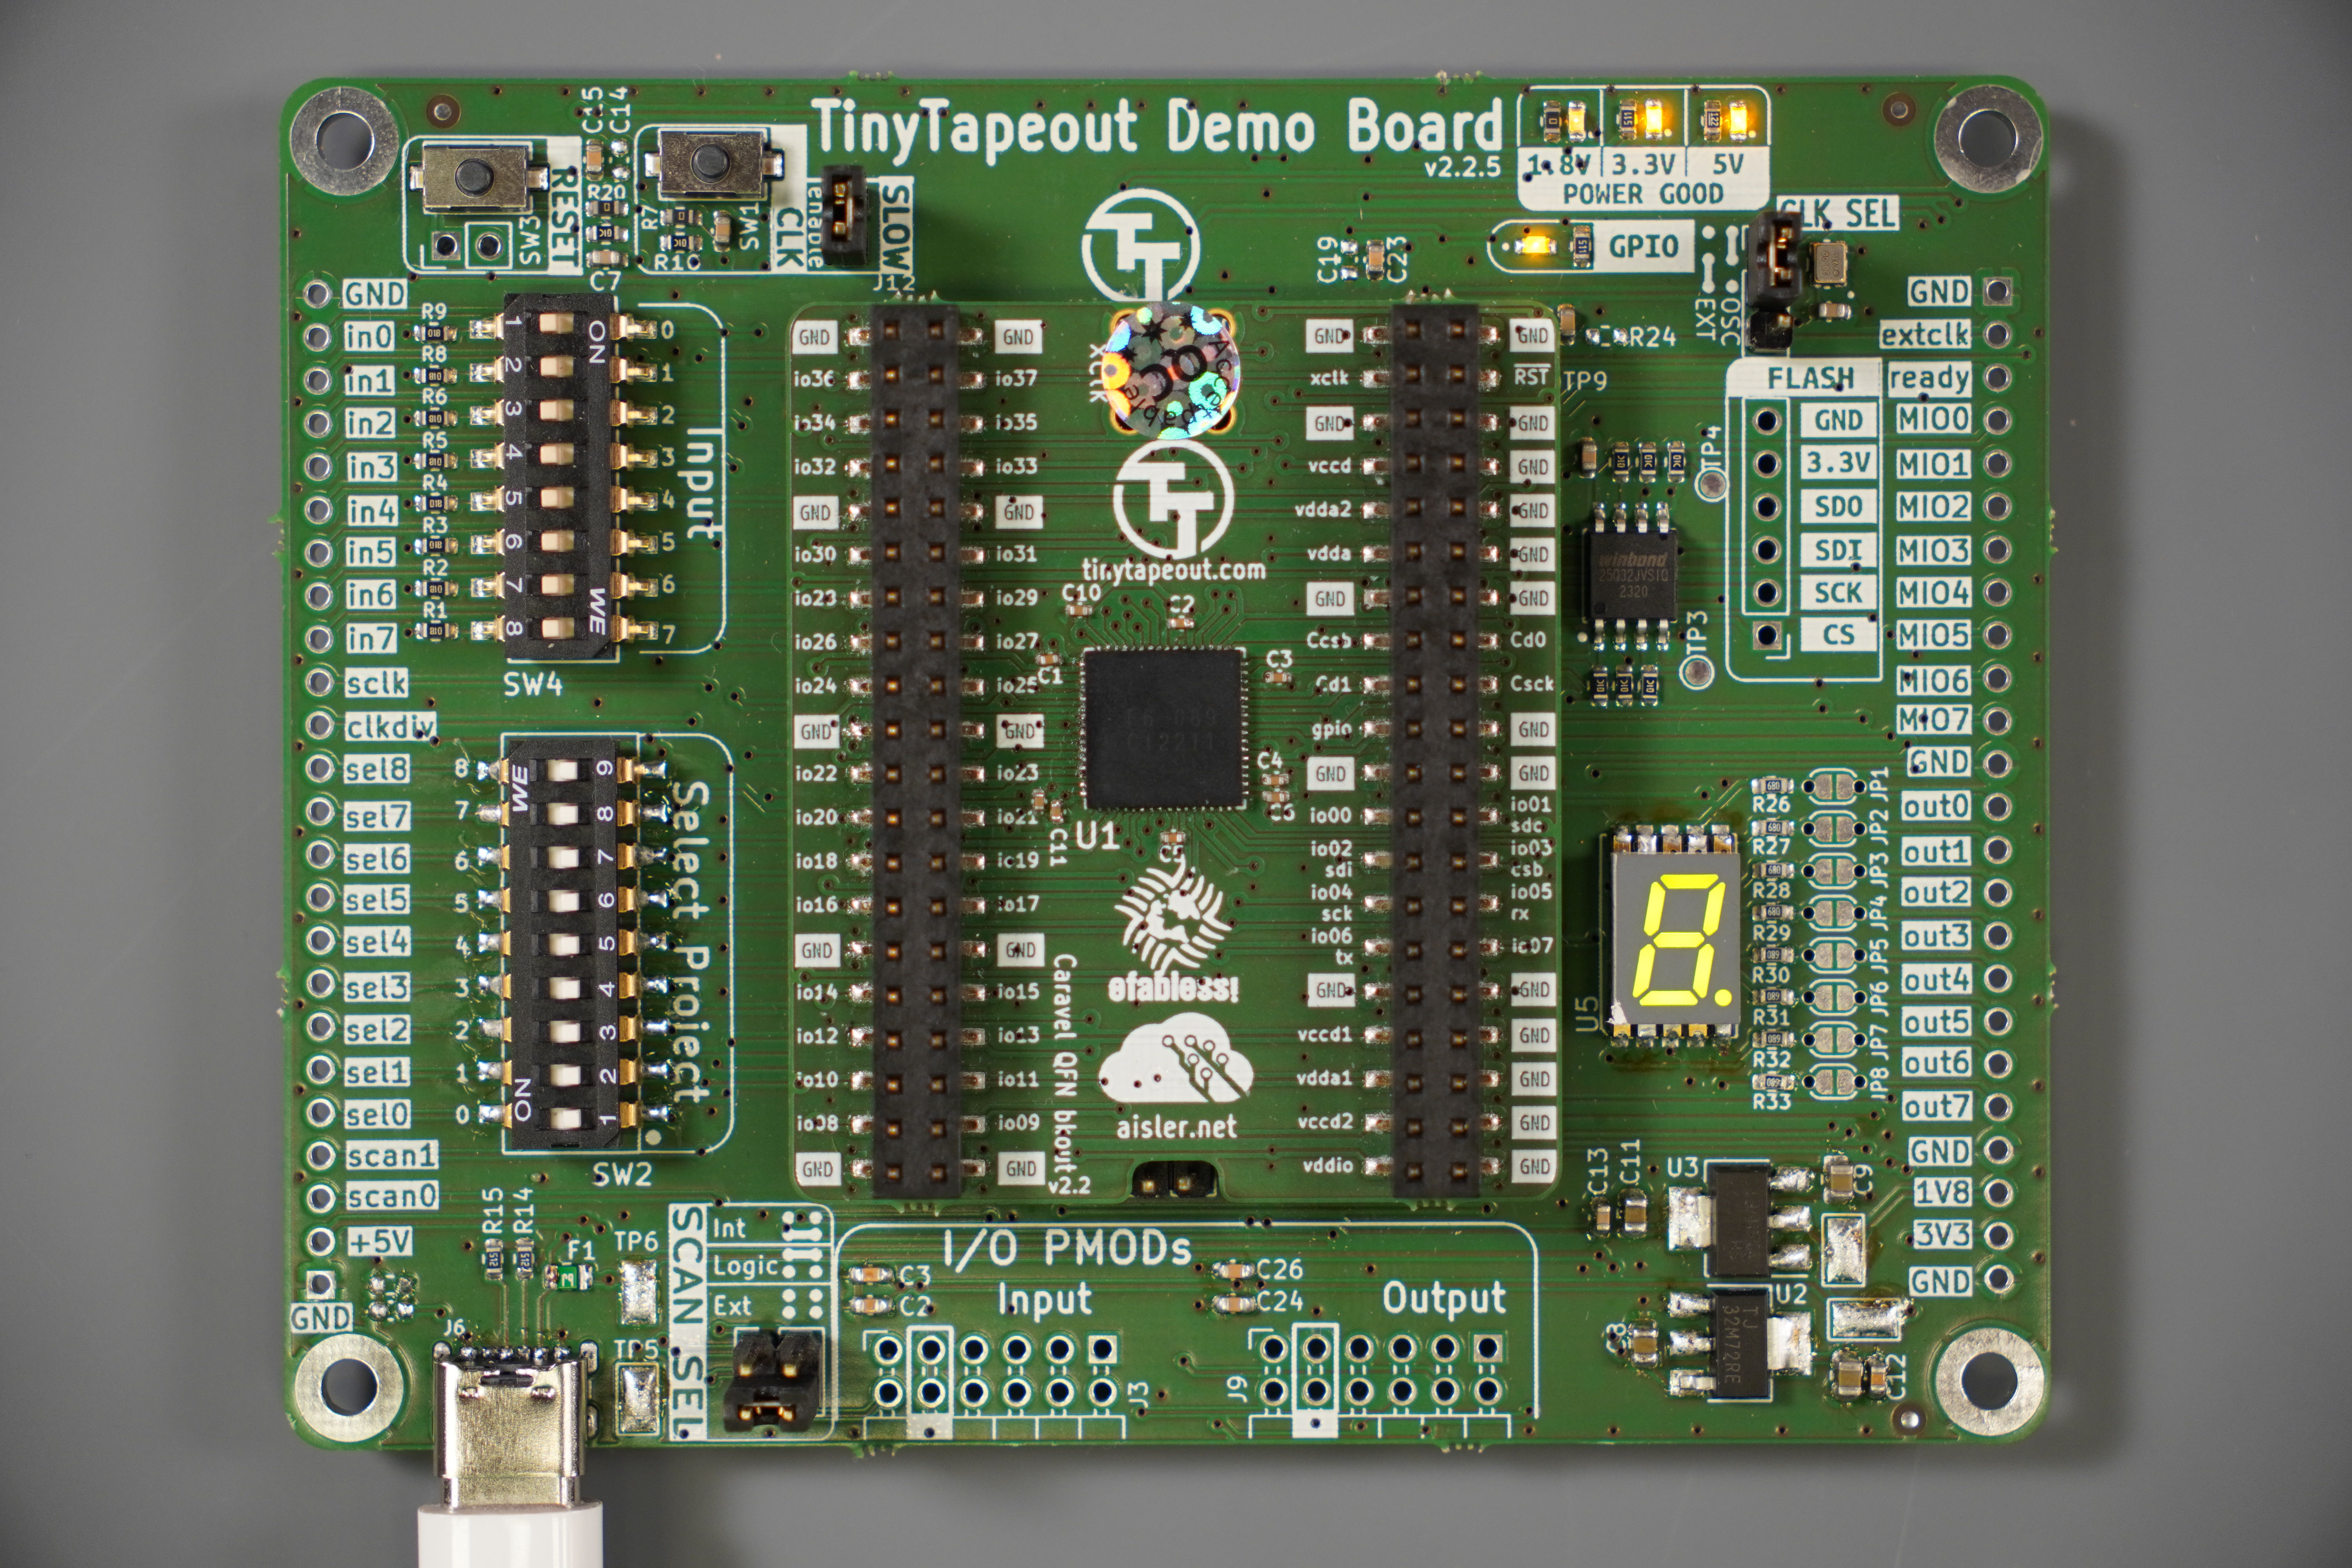
\includegraphics[width=0.5\textwidth]{./Figs/tt02 pcb assembled.JPG}
\caption{The demonstration board. Certified Open Source Hardware ES000040~\cite{oshwacertification}.}
\label{fig:demonstration_board}
\end{figure}

\section{Scan Chain Silicon Results}
\label{sec:scan_chain_res}

TT02 chips were received in October 2023, 11 months after the chips were submitted for manufacture on Efabless chipIgnite 2211Q.
The chips were tested for the first time in public on a livestream~\cite{siliconalive}.
The chain was validated, and a few of the designs were shown to be working.

\begin{figure}[!t]
\centering
\includegraphics[width=\columnwidth]{./Figs/tt02_clock_out.png}
\caption{Measurement from TT02 silicon, with input clock in yellow and the distorted output clock in blue.}
\label{fig:TT02_clock_out}
\end{figure}

In the following days another 30 designs were tested and shown to be working.

After measuring the clock asymmetry (Fig.~\ref{fig:TT02_clock_out}) and maximum frequency it was decided to run the production boards with a \qty{20}{\MHz} oscillator, resulting in a \qty{10}{\MHz} scan chain clock and a \qty{5}{\kHz} IO update rate.

Some designs didn’t function as expected, which in most cases was due to faults in the submitted design.

As well as 82 Verilog designs, 64 used the Wokwi graphical editor, 6 used alternative HDLs like VHDL, Amaranth~\cite{amaranth} and Chisel~\cite{chisel}.
Some Wokwi designs using combinational logic in clock paths (Fig.~\ref{fig:failed_design_comb_logic}) worked in simulation but failed in hardware.
This was due to the lack of timing data in the simulation, and wasn’t detected by STA because the clock paths were not known. A detailed analysis has yet to be carried out.

\begin{figure}[!t]
\centering
\includegraphics[width=\columnwidth]{./Figs/wokwi mux clock logic.png}
\caption{Combinational logic in the clock path of one of the failed designs.}
\label{fig:failed_design_comb_logic}
\end{figure}

At the time of writing, PCBs are in production and are expected to ship to customers by the end of January 2024.

Tiny Tapeout 3 silicon was received in January 2024, and the updated scan chain shows a more symmetric (Fig.~\ref{fig:TT03_silicon_measurement}) output clock at the end of the chain. This will allow a faster scan chain clock, resulting in a faster update frequency.

\begin{figure}[!t]
\centering
\includegraphics[width=\columnwidth]{./Figs/tt03_clock_out.png}
\caption{Measurement from TT03 silicon.}
\label{fig:TT03_silicon_measurement}
\end{figure}

\section{Beyond the Scanchain}
\label{sec:beyond_scanchain}
The biggest limitation of the Tiny Tapeout architecture was the IO bandwidth and latency.
For Tiny Tapeout 4 a new architecture was needed, and a series of proposals was gathered from the community.
An online video call was held and the 10 proposals discussed.
The winning design was a fairly straightforward multiplexer design shown in Fig.~\ref{fig:multiplexer_design}.

\begin{figure}[htp]
\centering
\includegraphics[width=\columnwidth]{./Figs/mux architecture.png}
\caption{Simplified diagram of the multiplexer architecture.}
\label{fig:multiplexer_design}
\end{figure}

The physical layout (shown in Fig.~\ref{fig:TT03_5_test_design}) consists of a central controller connected up and down to two vertical spines.
Twenty-four horizontal muxes connect to the spine with each supporting 16 designs.
This allows up to 384 separate single tile designs.
Multiple tile designs were also enabled, allowing a maximum project size of \(8 \times 2\) tiles or \(1359 \times 225 \mu m\) - around 20,000 logic cells.

\begin{figure}[htp]
\centering
\includegraphics[width=\columnwidth]{./Figs/tt3p5 layout.png}
\caption{The TT03.5 test design.}
\label{fig:TT03_5_test_design}
\end{figure}

Another major limitation of TT01 to TT03 was the small number of IO.
The scan controller used 9 GPIOs to select the currently active design, which, while simplifying the demo board, wasted valuable pins.
With TT04, the parallel design selection was dropped in favor of a serial protocol.
The extra pins were then used as bidirectional pins, giving each design clock, reset, and 24 IO.

\begin{table}[htp]
\centering
\caption{Comparison between TT03 and TT04}
\label{tab:comparison_TT03_TT04}
\begin{tabular}{@{}lcc@{}}
\toprule
Parameters & Tiny Tapeout 3 & Tiny Tapeout 4 \\
\midrule
Max clock speed & \(12.5 kHz\) & \(50 MHz\) \\
Max design size & \(150 \times 170 \mu m\) & \(1359 \times 225 \mu m\) \\
Input pins & \(8\) & \(10\) \\
Output pins & \(8\) & \(8\) \\
Bidirectional I/O pins & None & \(8\) \\
Custom GDS file & \xmark & \checkmark \\
\bottomrule
\end{tabular}
\end{table}

An invite-only experimental shuttle~\cite{tinytapeout03p5} was submitted with 32 designs to Efabless chipIgnite 2306C.
Two of the designs included a power gate as a stepping stone to supporting analog and mixed-signal designs.

\section{Multiplexer Silicon Results}
\label{sec:multiplexer_silicon_res}
After silicon was received, the worst round trip latency was measured to be \(20 ns\).

\begin{figure}[htp]
\centering
\includegraphics[width=\columnwidth]{./Figs/tt3p5 rising latency.PNG}
\caption{Round trip latency on a rising edge of about \(20 ns\).}
\label{fig:round_trip_latency_rising_edge}
\end{figure}

\begin{figure}[htp]
\centering
\includegraphics[width=\columnwidth]{./Figs/tt3p5 falling latency.PNG}
\caption{Round trip latency on a falling edge of about \(16 ns\).}
\label{fig:round_trip_latency_falling_edge}
\end{figure}

The new chip pinout and serial design selection required a new demo board that included an easy way to select the design.
The RP2040 microcontroller was chosen as a co-processor as it allows:
\begin{itemize}
\item Drag and drop firmware updates on any OS,
\item Runs MicroPython\cite{micropython}, ideal for beginners to test their designs,
\item External memory emulation via PIO and DMA.
\end{itemize}

\begin{figure}[htp]
\centering
\includegraphics[width=\columnwidth]{./Figs/tt3p5 enable design.png}
\caption{A MicroPython program enabling a design, clocking it, and printing the results.}
\label{fig:micropython_program}
\end{figure}

\begin{figure}[htp]
\centering
\includegraphics[width=\columnwidth]{./Figs/tt04-demoboard-top.jpg}
\caption{The TT04+ demo board.}
\label{fig:TT04plus_demo_board}
\end{figure}

An additional PMOD expansion port was added for the bidirectional pins, and the community has started to standardize on pinouts~\cite{pinouts} making it easier to test each other's designs.
A new repository was created to house user-contributed PMODs~\cite{awesomepmods}.

\begin{figure}[htp]
\centering
\includegraphics[width=\columnwidth]{./Figs/tiny_vga_pmod.jpg}
\caption{A user-contributed VGA output PMOD.}
\label{fig:user_contributed_VGA_PMOD}
\end{figure}

\begin{figure}[htp]
\centering
\includegraphics[width=\columnwidth]{./Figs/tt3p5 vga clock.jpg}
\caption{VGA clock design running on TT03.5 silicon.}
\label{fig:VGA_clock_design_TT03_5_silicon}
\end{figure}


\section{Improving the multiplexer and mixed signal support}
\label{sec:improving}

TT05 split the mux into two parts to improve performance.
As each spine segment is now half as long, it will have half the capacitance.
We expect to reduce the round trip latency to around \(10 ns\).

For TT06, the Caravel harness will be replaced by OpenFrame\cite{openframe}, an alternative harness provided by Efabless that uses the same padring but removes the RISC-V coprocessor.
This adds an extra \(5 mm^2\) more space for user designs, and an extra \(12\) pins that will be used for analog.

For increased safety, all designs will be power-gated, which will allow designers to take more risks or use custom flows.

Analog and mixed-signal designs will be enabled by adding an analog multiplexer based on transmission gates\cite{transmissiongates}. 
This allows up to \(192\) designs to share the \(8\) analog pins between them.
The transmission gates were tested as part of an experimental analog submission to TT05 shown in Fig.~\ref{fig:transmission_gate_TT05}.

\begin{figure}[htp]
\centering
\includegraphics[width=\columnwidth]{./Figs/tt05_transmission_gate.png}
\caption{Analog design submitted to TT05 with a transmission gate high-lighted (auto-placed and auto-routed using an experimental analog P&R tool).}
\label{fig:transmission_gate_TT05}
\end{figure}

TT06 is planned to open for digital designs at the end of January 2024, for analog designs at the end of February, and to close on April 19th, 2024.

\section{Silicon Showcase}
\label{sec:silicon_showcase}

A curated list showcasing the types of designs possible through Tiny Tapeout is provided below:

\begin{itemize}
    \item Serial FPGA~\cite{showcaseserialfpga}: a one fracturable 5-LUT that receives FPGA LUT configuration frames and serially evaluates LUT inputs and LUT outputs.
    \item Synthesizable digital temperature sensor~\cite{showcasetempsense}: a design which creatively twists the use of a tristate-inverter (EINVP) to create voltage  digital to analog converter (DAC). This voltage-mode DAC is used to bias an NMOS into subthreshold operation to discharge the input capacitor of an inverter. Since the subthreshold current of a MOSFET is a strong function of temperature, the resulting delay time is also a strong function of temperature, thus a digital temperature sensor is created.
    \item 395 standard cells with multiplexer~\cite{showcasemicrotapeout}: a design which contains a copy of most standard cells in the SkyWater sky130\_fd\_sc\_hd library along with a multiplexing mechanism that allows the user to expose any of them to the input/output pins.
    \item FM transmitter with I2S input~\cite{showcasefmtx}: a design which takes an audio signal and modulates it to a higher carrier frequency using frequency modulation (FM). The modulator in this design is based on a numerically controlled oscillator (NCO) with several modifications.
    \item USB Full Speed device~\cite{showcaseusb}: a hardware implementation of a USB Device hardware interface, designed to be compliant with USB1.1 Full Speed/Low Speed modes but not High Speed.
    \item A Linux capable RISC-V CPU~\cite{showcasekianv}: a functional RV32IMA RISC-V processor designed to boot and run the uLinux Linux distribution for resource constrained devices.
\end{itemize}

An index of all designs submitted to Tiny Tapeout can be found at \url{TinyTapeout.com/runs/}~\cite{tinytapeoutruns}.


% can remove
%\section{Conclusions}
\label{sec:conclusions}
The conclusion goes here.

\section{Acknowledgements}
\label{sec:acknowledgements}

\begin{enumerate}
    \item Uri Shaked for Wokwi development and lots more.
    \item Sylvain Munaut for help with scan chain improvements and multiplexer design.
    \item Mike Thompson and Mitch Bailey for verification expertise.
    \item Jix for formal verification support.
    \item Proppy for help with GitHub actions.
    \item Maximo Balestrini for the amazing renders and the interactive GDS viewer.
    \item Harald Pretl for advice and analog support.
    \item The team at YosysHQ and all the other open source EDA tool makers.
    \item Efabless for running the shuttles and providing OpenLane and sponsorship.
    \item Tim Ansell and Google for supporting the open source silicon movement.
    \item Pat Deegan for PCB development.
    \item The TinyTapeout community for all their contributions.
    \item The Zero to ASIC course community for all their support.
\end{enumerate}




%%%%%%%%% -- BIB STYLE AND FILE -- %%%%%%%%
\bibliographystyle{IEEEtran}
\bibliography{IEEEabrv,references.bib}
%%%%%%%%%%%%%%%%%%%%%%%%%%%%%%%%%%%%

\end{document}
